\section{Circuits}

\lipsum[1]

\begin{figure}[h]
    \centering
    \begin{circuitikz}
      \draw (0,0) to[V, label=4V] (0,2);
      \draw (0,2) -- (2,2);
      \draw (2,2) to[L, label=0.5H] (2,0) -- (0,0);
      \draw (2,2) -- (4,2);
      \draw (4,2) to[C, label=0.5$\mu$F] (4,0) -- (0,0);
    \end{circuitikz}
    \caption{Simple parallel circuit with a voltage source, inductor, and capacitor.}
    \label{fig:circuit}
\end{figure}


\begin{figure}[h]
    \centering
    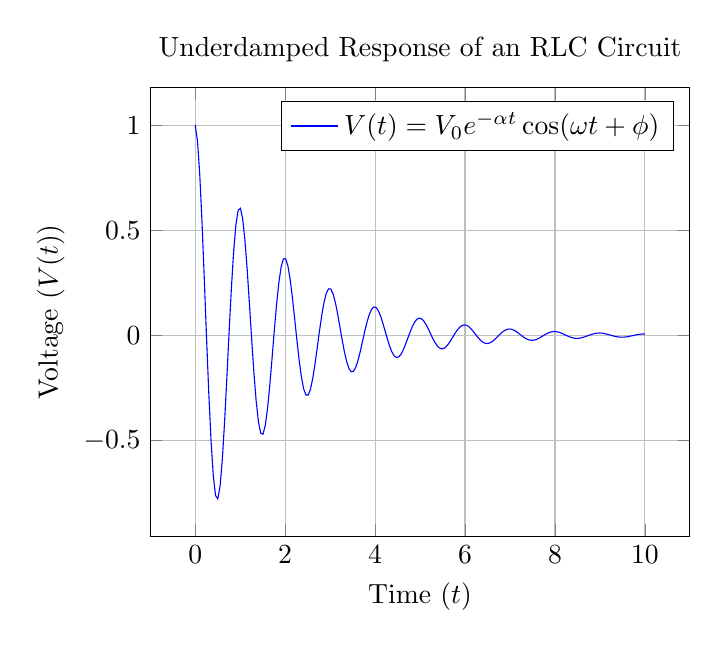
\begin{tikzpicture}
    
        \begin{axis}[
            title={Underdamped Response of an RLC Circuit},
            xlabel={Time (\(t\))},
            ylabel={Voltage (\(V(t)\))},
            grid=major,
            domain=0:10,
            samples=200,
            legend pos=north east,
        ]
        \addplot[blue] {exp(-0.5*x) * cos(deg(2*pi*x))};
        \legend{\(V(t) = V_0 e^{-\alpha t} \cos(\omega t + \phi)\)}
        \end{axis}
    \end{tikzpicture}
    \caption{Voltage Responce of Parrallel RLC circuit }
    \label{fig:underdampedgraph}
\end{figure}

In the text, you can refer to this figure as shown in Figure \ref{fig:circuit}. Figure \ref{fig:underdampedgraph} is there too.

\lipsum[1]

% \begin{figure}[h]
% \centering
% \includegraphics[width=10cm]{photos/1.4_1uf_scope.png}
% \caption{Your caption here.}
% \label{fig:your-label}
% \end{figure}

\newpage